% Gemini theme
% https://github.com/anishathalye/gemini

\documentclass[final]{beamer}

% ====================
% Packages
% ====================

\usepackage{xeCJK}
\setCJKmainfont{微軟正黑體}
\XeTeXlinebreaklocale "zh"
\XeTeXlinebreakskip = 0pt plus 1pt
\usepackage[T1]{fontenc}
\usepackage{lmodern}
\usepackage[size=custom,width=59.4,height=84.1,scale=1.0]{beamerposter}
\usetheme{gemini}
\usecolortheme{gemini}
\usepackage{graphicx}
\usepackage{booktabs}
\usepackage{tikz}
\usepackage{pgfplots}
\pgfplotsset{compat=1.14}
\usepackage{anyfontsize}
\usepackage{url}
\usepackage{subcaption}
\captionsetup[figure]{labelformat=simple, labelsep=colon}
\usepackage{etoolbox}
\newenvironment{subblock}[1]{%
  \begin{beamercolorbox}[sep=1em]{block body}%
  \textbf{#1}\par\vspace{0em}%
}{%
  \end{beamercolorbox}
}
\setbeamercolor{block body}{bg=gray!10,fg=black}
\usepackage{array}
\newcolumntype{L}[1]{>{\raggedright\arraybackslash}p{#1}}
% ====================
% Lengths
% ====================

% If you have N columns, choose \sepwidth and \colwidth such that
% (N+1)*\sepwidth + N*\colwidth = \paperwidth
\newlength{\sepwidth}
\newlength{\colwidth}
\setlength{\sepwidth}{0.025\paperwidth}
\setlength{\colwidth}{0.4625\paperwidth}

\newcommand{\separatorcolumn}{\begin{column}{\sepwidth}\end{column}}

% ====================
% Title
% ====================

\title{Offloading and Quantizing LLaMA-3.1-8B for Resource-Constrained Inference on NVIDIA RTX 3060 Ti}
\author{111550165 吳宗樺, 111550087 林炫廷}

% ====================
% Footer (optional)
% ====================

\footercontent{
  }
% (can be left out to remove footer)

% ====================
% Logo (optional)
% ====================

% use this to include logos on the left and/or right side of the header:
% \logoright{\includegraphics[height=7cm]{logo1.pdf}}
% \logoleft{\includegraphics[height=7cm]{logo2.pdf}}

% ====================
% Body
% ====================

\begin{document}

\begin{frame}[t]
\begin{columns}[t]
 % Left separator
 \separatorcolumn

 % First zone: Setup and Implementation
 \begin{column}{\colwidth}
    \begin{block}{Abstract}
      \textbf{\textcolor{blue}{Large language models (LLMs)}} like \textbf{LLaMA-3.1-8B} present substantial \textcolor{blue}{memory constraints}, limiting deployment on resource-constrained hardware. We explore strategies to enable efficient inference of LLaMA-3.1-8B on an \textbf{NVIDIA RTX 3060 Ti GPU}, which lacks sufficient VRAM for standard model execution.

We begin by attempting to load the model in full precision, which immediately triggers \textbf{Out-of-Memory (OOM)} errors. To address this, we apply:

\vspace{-0.5em}
\begin{itemize}
  \item \textbf{\textcolor{red}{Post-training quantization}}: Compressing the model by reducing weight precision (e.g., from FP32 to INT8 or INT4) without retraining.
  \item \textbf{\textcolor{red}{Mixed-precision quantization}}: Using different bit-widths (e.g., 8-bit for critical layers, 4-bit elsewhere) to balance efficiency and accuracy.
  \item \textbf{\textcolor{red}{Dynamic offloading}}: Actively transferring non-critical tensors (e.g., key-value cache) between GPU VRAM and CPU RAM/disk to fit large models on limited-memory GPUs.
\end{itemize}
\vspace{-0.5em}

\begin{figure}
  \centering
  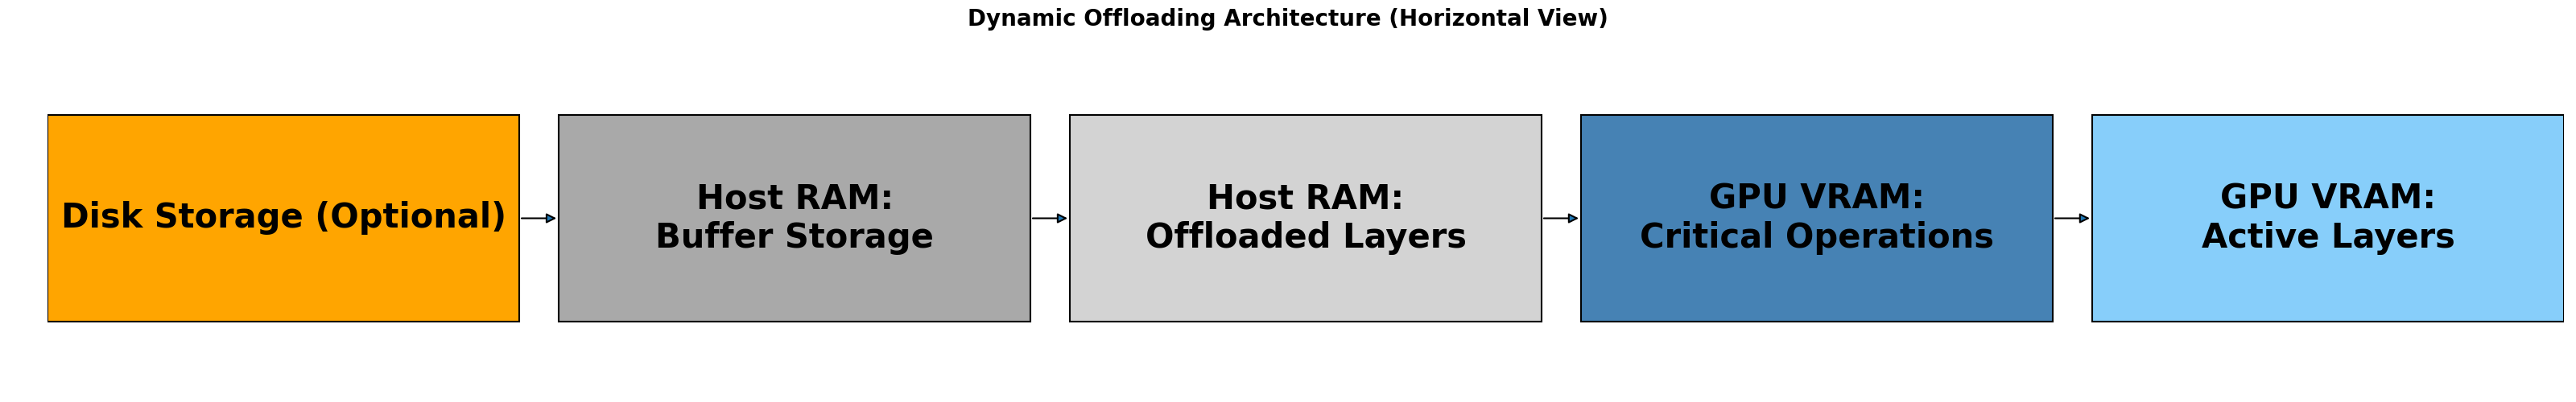
\includegraphics[width=1\colwidth]{dynamic_offloading_architecture.png}
  \caption{Illustration of dynamic offloading across memory hierarchies during inference.}
  \label{fig:llama_model}
\end{figure}
    \end{block}   
    \begin{block}{Model Architecture}
      \begin{itemize}
        \item \textbf{Model}: LLaMA-3.1-8B
        \item \textbf{Architecture}: Transformer-based architecture with 8 billion parameters
        \item \textbf{Layers}: 32 transformer layers
        \item \textbf{Hidden Size}: 5120
        \item \textbf{Activation Function}: GeLU (Gaussian Error Linear Unit)
        
      \end{itemize}
      \begin{figure}
        \begin{subfigure}{0.48\colwidth}
          \centering
          \includegraphics[width=0.2\colwidth]{high\_level\_architecture.png}
          \caption{The overview of LLaMA-3.1-8B architecture.}
          \label{fig:llama_sturcture}
        \end{subfigure}
        \hfill
        \begin{subfigure}{0.48\colwidth}
          \centering
          \includegraphics[width=0.2\colwidth]{decoder\_layer\_detail.png}
          \caption{Layer-wise parameter distribution in LLaMA-3.1-8B.}
          \label{fig:decode_layer}
        \end{subfigure}
        \caption{LLaMA-3.1-8B architecture and layer-wise parameter distribution.}
      \end{figure}
  \end{block}
  \begin{block}{References}
    \vspace{0.5em}
     [1] Zhihang Yuan et al., "LLM Inference Unveiled: Survey and Roofline Model Insights," arXiv:2402.16363, 2024.\\ {}
     [2] Amir Gholami et al., "A Survey of Quantization Methods for Efficient Neural Network Inference," arXiv:2103.13630, 2021.\\ {}
     [3] Ying Sheng et al., "FlexGen: High-Throughput Generative Inference of Large Language Models with a Single GPU," arXiv:2303.06865, 2023.\\ {}
     [4] Woosuk Kwon et al., "Efficient Memory Management for Large Language Model Serving with PagedAttention," arXiv:2309.06180, 2023.\\ {}
     [5] Wu et al., Prediction-Difference Quantization (PD-Quant), " arXiv:2212.07048, 2023. \\ {}
     \vspace{0.5em}
  \end{block}
 \end{column}

 % Middle separator
 \separatorcolumn

 % Second zone: Results and Analysis
 \begin{column}{\colwidth}
  \begin{block}{Preliminary Attempt}
    We attempted to load the full-precision LLaMA-3.1-8B on RTX 3060 Ti immediately triggered CUDA OOM errors, confirming that direct inference is infeasible without optimization.
    \begin{figure}
      \centering
      \includegraphics[width=0.5\colwidth]{full\_size\_model.png}
      \caption{LLaMA-3.1-8B model architecture and parameter distribution.}
      \label{fig:model}
    \end{figure}
  \end{block}
  \vspace{-1em}

  \begin{block}{Experiment}
    To evaluate the impact of quantization and offloading strategies on Llama-3.1-8B inference, 
    we conduct experiments on an NVIDIA 3060 Ti GPU.
    We assess performance based on:
    \vspace{-0.5em}
    \begin{itemize}
      \item \textbf{OOM(Out of memory) Error}: The system (usually CPU or GPU) runs out of available memory to store or compute data
      \item \textbf{Inference Time}: Time taken to process a batch of inputs (in seconds)
      \item \textbf{Perplexity}: Language model evaluation metric (lower is better)
    \end{itemize}
    \vspace{-0.5em}
    \begin{table}
      \centering
      \caption{Performance metrics for LLaMA-3.1-8B with base configurations.}
      \fontsize{16}{8.2}
      \begin{tabular}{@{}L{15cm}ccc@{}}
        \toprule
        \textbf{Configuration} & \textbf{OOM Error} & \textbf{Inference Speed (s)} & \textbf{Perplexity}\\
        \midrule
        Full-precision Model (FP32) & Yes & N/A & N/A\\
        Baseline (PTQ with INT8) & No & 33.320 & 7.293 \\
        \bottomrule
    \end{tabular}
    \end{table}
   \end{block}

  \begin{subblock}{Dynamic Offloading}
    \begin{table}
      \centering
      \caption{Performance metrics for LLaMA-3.1-8B with offloading configurations.}
      \fontsize{16}{8.2}
      \begin{tabular}{@{}L{15cm}ccc@{}}
        \toprule
        \textbf{Configuration} & \textbf{OOM Error} & \textbf{Inference Speed (s)} & \textbf{Perplexity}\\
        \midrule
        HuggingFace's Offloading & No & 205.508 & 9075.724\\
        Our Offloading Strategy  & No & 159.728 & 7.234 \\
        \bottomrule
    \end{tabular}
    \end{table}
  \end{subblock}
  \par\vspace{1em}
  \begin{subblock}{Mixed-Precision Quantization With Offloading}
    \begin{table}
      \centering
      \caption{Performance metrics for LLaMA-3.1-8B with our configurations.}
      \fontsize{16}{8.2}
      \begin{tabular}{@{}L{15cm}ccc@{}}
        \toprule
        \textbf{Configuration} & \textbf{OOM Error} & \textbf{Inference Speed (s)} & \textbf{Perplexity}\\
        \midrule
        Mixed Precision + Our Offloading Strategy & No & 33.320 & 7.293\\
        Mixed Precision (8b L4 \& L7, 4b elsewhere) & No & 13.141 & 7.291 \\
        \bottomrule
    \end{tabular}
    \end{table}
  \end{subblock}
  \vspace{-1em}

 \begin{block}{Conclusion}
  We explored the feasibility of running the Llama-3.1-8B model on limited GPU resources using quantization and offloading techniques. 
  These results highlight the practicality of combining quantization and offloading for resource-constrained environments. 
  \end{block}
  \begin{block}{Future Improvements}
    We aim to extend our work along several directions:
    \vspace{-0.5em}

    \begin{itemize}
        \item \textbf{Larger Model Experiments}
        \begin{itemize}
            \item Test Llama-3.1-13B model with quantization and offloading.
        \end{itemize}
    
        \item \textbf{Hardware Deployment}
        \begin{itemize}
            \item Re-run all experiments directly on other GPU-insufficient hardware, like embedded systems.
            \item Take more different configure and compare their speed, memory usage, and performance.
        \end{itemize}
    \end{itemize}
    \vspace{0.35em}
  \end{block}

 \end{column}
 
 % Right separator
 \separatorcolumn
\end{columns}
\end{frame}

\end{document}
